\documentclass[12pt]{article}
\usepackage[ukrainian,shorthands=off]{babel}   % shorthands=off: символ " не активний (потрібно для міток "..." у TikZ всередині \zadtask)
\usepackage{fontspec}
% --- НАЛАШТУВАННЯ ШРИФТІВ ---
% Шрифти Schoolbook-*.otf лежать у корені проєкту. Шлях підбирається автоматично:
% ../ (компіляція з папки теми), ./ (корінь проєкту), ../../ (підпапки теми 28); інакше -- TeX Gyre Schola.
\newcommand{\nmtSchoolbook}[1]{\setmainfont{Schoolbook-Regular.otf}[
    Path = #1,
    BoldFont = Schoolbook-Bold.otf,
    ItalicFont = Schoolbook-Italic.otf,
    BoldItalicFont = Schoolbook-BoldItalic.otf
]}
\IfFileExists{../Schoolbook-Regular.otf}{\nmtSchoolbook{../}}{%
 \IfFileExists{./Schoolbook-Regular.otf}{\nmtSchoolbook{./}}{%
  \IfFileExists{../../Schoolbook-Regular.otf}{\nmtSchoolbook{../../}}{%
   \setmainfont{texgyreschola}[Extension=.otf, UprightFont=*-regular, BoldFont=*-bold, ItalicFont=*-italic, BoldItalicFont=*-bolditalic]}}}
\usepackage[italic]{mathastext}
\usepackage[a4paper,margin=1.8cm,bottom=2cm,top=2cm]{geometry}
\usepackage{amsmath,amssymb}
\usepackage{tikz}
\usepackage{pgfplots}
\pgfplotsset{compat=1.18}
\usepgfplotslibrary{fillbetween}
\usetikzlibrary{calc,patterns,angles,quotes,intersections,babel,3d,shapes.symbols,shapes.geometric,decorations.pathreplacing,shadings,arrows.meta,hobby}
\usepackage{xcolor,array,fancyhdr,enumitem,multicol}
\usepackage{colortbl,multirow,diagbox,needspace}
\usepackage{tcolorbox}
\tcbuselibrary{skins,breakable}
\usepackage[hidelinks]{hyperref}
% водяний знак; щоб зібрати без нього (версія для вчителів), перед \documentclass пишуть \def\nmtnowatermark{}
\ifdefined\nmtnowatermark\else
\usepackage[firstpage=false, text=@pvtr2525, scale=0.6, color=gray!12]{draftwatermark}
\fi

% --- АВТОСТИСКАННЯ: рисунок/сітка, ширша за колонку, масштабується до ширини колонки ---
\newsavebox{\nmtfitbox}
\newenvironment{nmtfit}{\begin{lrbox}{\nmtfitbox}}{\end{lrbox}%
  \ifdim\wd\nmtfitbox>\linewidth \resizebox{\linewidth}{!}{\usebox{\nmtfitbox}}\else\usebox{\nmtfitbox}\fi}
\let\nmtIncludegraphicsOrig\includegraphics
\renewcommand{\includegraphics}[2][]{\begin{nmtfit}\nmtIncludegraphicsOrig[#1]{#2}\end{nmtfit}}


\definecolor{mainGreen}{RGB}{34, 120, 64}
\definecolor{yearOrange}{RGB}{220, 100, 30}
\definecolor{yearcolor}{RGB}{220, 100, 30}
\definecolor{titleBg}{RGB}{225, 240, 220}
\definecolor{instrBg}{RGB}{255, 240, 220}
\definecolor{instrBorder}{RGB}{220, 150, 80}
\definecolor{headerblue}{RGB}{0, 102, 204}   % використовується в рисунках старої бази

\setlength{\parindent}{0pt}
\emergencystretch=1.5em

\pagestyle{fancy}
\fancyhf{}
\renewcommand{\headrulewidth}{0.4pt}
\renewcommand{\footrulewidth}{0.4pt}
\fancyhead[C]{\small\color{gray!80} Варіант № 2}
\fancyhead[R]{\small\color{mainGreen}\textbf{\href{https://t.me/pvtr2525}{@pvtr2525}}}
\fancyfoot[L]{\small\color{gray!80}\href{https://t.me/pvtr2525}{ТГ: @pvtr2525}}
\fancyfoot[C]{\small\color{gray!80}\thepage}
\fancyfoot[R]{\small\color{gray!80}НМТ з математики}

% --- ТАБЛИЦІ ВІДПОВІДЕЙ ---
% ширина клітинки = (ширина рядка - відступи) / 5: на всю сторінку це ~3 см, у minipage поруч із рисунком таблиця стискається
\newlength{\nmtcellw}
\newcommand{\nmtSetCell}{\setlength{\nmtcellw}{\dimexpr(\linewidth-12\tabcolsep-6\arrayrulewidth)/5\relax}}
\newcommand{\answerTable}[5]{%
\par\nopagebreak\vspace{0.15cm}
\noindent\nmtSetCell
\begin{tabular}{|*{5}{>{\centering\arraybackslash}m{\nmtcellw}|}}
\hline
\rule[-0.15cm]{0pt}{0.6cm}\textbf{А} & \rule[-0.15cm]{0pt}{0.6cm}\textbf{Б} & \rule[-0.15cm]{0pt}{0.6cm}\textbf{В} & \rule[-0.15cm]{0pt}{0.6cm}\textbf{Г} & \rule[-0.15cm]{0pt}{0.6cm}\textbf{Д} \\
\hline
\rule[-0.2cm]{0pt}{0.75cm}#1 & \rule[-0.2cm]{0pt}{0.75cm}#2 & \rule[-0.2cm]{0pt}{0.75cm}#3 & \rule[-0.2cm]{0pt}{0.75cm}#4 & \rule[-0.2cm]{0pt}{0.75cm}#5 \\
\hline
\end{tabular}
\par\vspace{0.25cm}
}
\newcommand{\answerTableTall}[5]{%
\par\nopagebreak\vspace{0.15cm}
\noindent\nmtSetCell
\begin{tabular}{|*{5}{>{\centering\arraybackslash}m{\nmtcellw}|}}
\hline
\rule[-0.2cm]{0pt}{0.7cm}\textbf{А} & \rule[-0.2cm]{0pt}{0.7cm}\textbf{Б} & \rule[-0.2cm]{0pt}{0.7cm}\textbf{В} & \rule[-0.2cm]{0pt}{0.7cm}\textbf{Г} & \rule[-0.2cm]{0pt}{0.7cm}\textbf{Д} \\
\hline
\rule[-0.45cm]{0pt}{1.2cm}#1 & \rule[-0.45cm]{0pt}{1.2cm}#2 & \rule[-0.45cm]{0pt}{1.2cm}#3 & \rule[-0.45cm]{0pt}{1.2cm}#4 & \rule[-0.45cm]{0pt}{1.2cm}#5 \\
\hline
\end{tabular}
\par\vspace{0.25cm}
}
\newcommand{\instructionBox}[1]{%
\par\vspace{0.3cm}
\begin{tcolorbox}[colback=instrBg, colframe=instrBorder, boxrule=0.6pt, arc=2pt,
    left=8pt, right=8pt, top=4pt, bottom=4pt]
\centering\small\bfseries #1
\end{tcolorbox}
\par\vspace{0.15cm}
}
\newcommand{\sectionTitle}[1]{%
\par\vspace{0.4cm}
\begin{tcolorbox}[colback=titleBg, colframe=titleBg, boxrule=0pt, arc=8pt,
    halign=center, fontupper=\Large\bfseries\color{mainGreen}]
\hyphenpenalty=10000 \exhyphenpenalty=10000 #1
\end{tcolorbox}
\par\vspace{0.3cm}
}
\newcommand{\task}[2]{\noindent\textbf{#1.}\ \ #2\par\vspace{0.2cm}}
% --- НМТ-СТИЛЬ ПОЛЕ ВІДПОВІДІ ---
\newcommand{\nmtAnswerBox}{%
\par\nopagebreak\vspace{0.2cm}\noindent
Відповідь:\ \
\begin{tabular}{@{}*{4}{|>{\centering\arraybackslash}p{0.8cm}}|@{\hspace{0.1cm}\textbf{,}\hspace{0.1cm}}*{3}{|>{\centering\arraybackslash}p{0.8cm}}|@{}}
\hline
\rule[-0.2cm]{0pt}{0.7cm} & & & & & & \\
\hline
\end{tabular}
\par\vspace{0.3cm}
}
% --- СІТКА ДЛЯ МАТЧИНГУ ---
\newsavebox{\nmtgridbox}
\newcommand{\matchingGrid}{%
    \sbox{\nmtgridbox}{\matchingGridRaw}%
    \ifdim\wd\nmtgridbox>\linewidth \resizebox{\linewidth}{!}{\usebox{\nmtgridbox}}\else\usebox{\nmtgridbox}\fi}
\newcommand{\matchingGridRaw}{%
    \begingroup
    \renewcommand{\arraystretch}{1.15}
    \setlength{\tabcolsep}{4pt}
    \footnotesize
    \begin{tabular}{r|c|c|c|c|c|}
         \multicolumn{1}{c}{} & \multicolumn{1}{c}{\textbf{А}} & \multicolumn{1}{c}{\textbf{Б}} & \multicolumn{1}{c}{\textbf{В}} & \multicolumn{1}{c}{\textbf{Г}} & \multicolumn{1}{c}{\textbf{Д}} \\ \cline{2-6}
         \textbf{1} & \phantom{X} & \phantom{X} & \phantom{X} & \phantom{X} & \phantom{X} \\ \cline{2-6}
         \textbf{2} & & & & & \\ \cline{2-6}
         \textbf{3} & & & & & \\ \cline{2-6}
    \end{tabular}
    \endgroup
}
% --- ДОДАТКОВІ МАКРОСИ ЗБІРНИКА ---
\newcommand{\taskBlock}[1]{%
\par\vspace{0.45cm}
\noindent{\color{mainGreen}\rule{\linewidth}{0.8pt}}\par\vspace{0.12cm}
\noindent{\small\bfseries\color{mainGreen}#1}\par\vspace{0.25cm}
}
\newcounter{zad}
\newcommand{\zadtask}[1]{\stepcounter{zad}\noindent\textbf{\thezad.}\ \ #1\par\nopagebreak\vspace{0.2cm}}
\newcommand{\zadnum}{\stepcounter{zad}\textbf{\thezad.}\ \ }
\newcounter{ans}
\newcommand{\ansitem}[1]{\stepcounter{ans}\noindent\textbf{\theans.}\ #1\par\vspace{0.07cm}}
% мітка року: нерозривна, притиснута праворуч; якщо не вміщається -- праворуч на новому рядку
\newcommand{\nmtyear}[1]{\unskip\nobreak\finalhyphendemerits=0 \hfill\penalty100\hskip1em\hbox{}\nobreak\hfill{\small\color{yearOrange}\mbox{\rule{0pt}{2.3ex}(НМТ~#1)}}}
% --- МАКРОС КОРОТКОГО РОЗВ'ЯЗКУ ---
\newcommand{\solution}[1]{%
\par\vspace{0.12cm}
\begin{tcolorbox}[colback=titleBg!45, colframe=mainGreen!55, boxrule=0.4pt, arc=2pt,
    left=6pt, right=6pt, top=3pt, bottom=3pt, breakable]
\footnotesize\textbf{Короткий розв'язок.}\ #1
\end{tcolorbox}
\par\vspace{0.12cm}
}
% Розв'язки й відповіді (є до завдань НМТ-2026): \showsolutionstrue -- показати, \showsolutionsfalse -- сховати
\newif\ifshowsolutions
\showsolutionsfalse
% --- ЗАГОЛОВКИ З ПУНКТАМИ КЛІКАБЕЛЬНОГО ЗМІСТУ ---
\setcounter{tocdepth}{2}
\newcommand{\chapterTitle}[1]{%
\clearpage\phantomsection\addcontentsline{toc}{section}{#1}%
\sectionTitle{#1}}
\newcommand{\typeTitle}[1]{%
\needspace{6\baselineskip}%
\phantomsection\addcontentsline{toc}{subsection}{\quad #1}%
\par\vspace{0.3cm}
\noindent{\large\bfseries\color{yearOrange}#1}\par\vspace{0.08cm}
\noindent{\color{yearOrange}\rule{\linewidth}{0.4pt}}\par\nopagebreak\vspace{0.2cm}}
\raggedbottom
% усередині одного завдання сторінка не розривається: нерозривний вертикальний проміжок
% і нерозривна межа абзаців (умова ніколи не відділяється від варіантів, рисунка чи сітки)
\newcommand{\nbvspace}[1]{\nopagebreak\vspace{#1}}
\newcommand{\nmtnobreak}{\ifvmode\penalty10000 \fi}
% --- ЄДИНИЙ МАКЕТ ЗАВДАНЬ НА ВІДПОВІДНІСТЬ ---
% мітка в колонці сталої ширини, текст -- у parbox: продовження довгого рядка
% вирівнюється під текстом, а не під міткою; відступ між пунктами однаковий скрізь
\newlength{\nmtMatchLab}\setlength{\nmtMatchLab}{1.6em}
\newlength{\nmtMatchSep}\setlength{\nmtMatchSep}{0.28cm}
\newcommand{\matchHead}[1]{\par\noindent\textit{#1}\par\nopagebreak\vspace{0.2cm}}
\newcommand{\matchItem}[2]{\par\noindent\makebox[\nmtMatchLab][l]{\textbf{#1}}%
\parbox[t]{\dimexpr\linewidth-\nmtMatchLab\relax}{\raggedright #2}\par\nopagebreak\vspace{\nmtMatchSep}}
\newcommand{\ansTheme}[1]{\par\vspace{0.25cm}\noindent{\bfseries\color{mainGreen}#1}\par\vspace{0.12cm}}
\newcommand{\ansType}[1]{\par\vspace{0.1cm}\noindent{\itshape\color{yearOrange}#1}\par\vspace{0.08cm}}

\graphicspath{{../1. Числа. Звичайні та десяткові дроби. Модуль числа/}{../10. Основи планіметрії/}{../11. Трикутники/}{../12. Паралелограм/}{../13. Прямокутник/}{../14. Квадрат/}{../15. Ромб/}{../16. Трапеція/}{../17. Коло, круг і їх елементи/}{../18. Координати і вектори на площині і в просторі. Рівняння кола/}{../19. Лінійні та квадратні нерівності. Системи лінійних нерівностей. Метод інтервалів/}{../2.відсотки, арифметичні задачі, подільність/}{../20. Функція та її властивості/}{../21.  Графіки елементарних функцій, їх побудова графіків функцій та їх перетворення/}{../22. Модульні  рівняння та нерівності/}{../23. Ірраціональні рівняння та нерівності/}{../24. Арифметична прогресія/}{../25. Геометрична прогресія/}{../26. Тригонометричні вирази/}{../27. Тригонометричні рівняння/}{../28. Показникова функція. Показникові рівняння/Показникові рівняння/}{../28. Показникова функція. Показникові рівняння/Показникові функція і вирази/}{../29. Показникові нерівності/}{../3. Степені. Одночлени. стандартний вигляд числа/}{../30. Логарифм. Логарифмічна функція/}{../31. Логарифмічні рівняння/}{../32. Логарифмічні нерівності/}{../33. Похідна/}{../34. Первісна/}{../35. Комбінаторика/}{../36. Теорія ймовірності/}{../37. Статистика/}{../38. Призма. Паралелепіпед. Куб/}{../39. Піраміда/}{../4.Многочлени. ФСМ/}{../40. Циліндр/}{../41. Конус/}{../42. Куля. Сфера/}{../43. Параметри/}{../5. дробові раціональні вирази і перетворення/}{../6. Лінійні рівняння/}{../7. Квадратні корені. Корені вищих степенів. Раціональний степінь/}{../8. квадратні рівняння, і рівняння, що до них зводяться/}{../9. Системи рівнянь/}}

\begin{document}
% макроси бази, потрібні аналогам
% --- сумісність зі старою базою (діє, якщо тема не має власного визначення) ---
\providecommand{\trigStyle}[1]{#1}
\providecommand{\answerTableSmall}[5]{%
\begingroup\setlength{\tabcolsep}{2pt}\small\nmtSetCell
\begin{tabular}{|*{5}{>{\centering\arraybackslash}m{\nmtcellw}|}}
\hline
\rule[-0.2cm]{0pt}{0.6cm}\textbf{А} & \textbf{Б} & \textbf{В} & \textbf{Г} & \textbf{Д} \\
\hline
\rule[-0.4cm]{0pt}{0.9cm}#1 & \rule[-0.4cm]{0pt}{0.9cm}#2 & \rule[-0.4cm]{0pt}{0.9cm}#3 & \rule[-0.4cm]{0pt}{0.9cm}#4 & \rule[-0.4cm]{0pt}{0.9cm}#5 \\
\hline
\end{tabular}\endgroup}
\providecommand{\matchingLayout}[3]{%
    \noindent
    \begin{minipage}[t]{0.36\textwidth}\vspace{0pt}\raggedright
        #1
    \end{minipage}%
    \hfill
    \begin{minipage}[t]{0.43\textwidth}\vspace{0pt}\raggedright
        #2
    \end{minipage}%
    \hfill
    \begin{minipage}[t]{0.19\textwidth}
        \vspace{0pt}
        \begin{flushright}
        #3
        \end{flushright}
    \end{minipage}}
\providecommand{\matchingLayoutBottom}[2]{%
    \noindent
    \begin{minipage}[t]{0.48\textwidth}\vspace{0pt}\raggedright
        #1
    \end{minipage}%
    \hfill
    \begin{minipage}[t]{0.48\textwidth}\vspace{0pt}\raggedright
        #2
    \end{minipage}
    \vspace{0.5cm}
    \noindent
    \matchingGrid}
\providecommand{\answerListVertical}[5]{%
    \par\nopagebreak\vspace{0.2cm}
    \begin{itemize}[itemsep=0.4cm, leftmargin=1.5cm, labelsep=0.5cm]
        \item[\textbf{А}] #1
        \item[\textbf{Б}] #2
        \item[\textbf{В}] #3
        \item[\textbf{Г}] #4
        \item[\textbf{Д}] #5
    \end{itemize}
    \vspace{0.2cm}}
\setcounter{zad}{0}

\chapterTitle{Тренувальний варіант НМТ з математики № 2}

\noindent{\small Варіант складено за структурою НМТ 2023--2026: 15 завдань з вибором однієї відповіді, 3 на встановлення відповідності й 4 з короткою відповіддю (максимум 32 бали). 14 завдань -- справжні завдання НМТ 2023--2026 років, 8 -- авторські аналоги таких самих завдань. Відповіді -- на останній сторінці.}\par\vspace{0.4cm}

\instructionBox{Завдання 1--15 мають по п'ять варіантів відповіді, з яких лише \textbf{один правильний}. Виберіть правильний, на Вашу думку, варіант відповіді й позначте його в бланку відповідей.}

\begin{samepage}
\zadtask{Потяг долає відстань між двома містами за $3$~год. Після ремонту колії середню швидкість потяга на цьому маршруті збільшили в $1{,}2$ раза. Скільки \textit{хвилин} тепер триватиме ця поїздка?}
\answerTable{$30$}{$144$}{$150$}{$170$}{$216$}
\par\penalty-20
\end{samepage}

\begin{samepage}
\noindent
\begin{minipage}[c]{0.46\textwidth}
\zadnum На рисунку зображено графік зміни температури $T$ (у $^\circ$C) повітря протягом доби. Скільки всього годин за добу температура повітря зростала?
\end{minipage}
\hfill
\begin{minipage}[c]{0.52\textwidth}
\centering
\begin{nmtfit}\begin{tikzpicture}[x=0.3cm, y=0.3cm, thick]
    \draw[step=2, gray!40, thin] (0,-4) grid (24,8);
    \draw[->] (-1,0) -- (26.5,0) node[right, font=\scriptsize] {$t$, год};
    \draw[->] (0,-4.5) -- (0,9) node[above, font=\scriptsize] {$T$, $^\circ$C};
    \node[below left, font=\scriptsize] at (0,0) {$0$};
    \foreach \x in {4,6,14,16,20,22,24} {
        \node[below, font=\scriptsize, inner sep=1pt] at (\x,-0.15) {$\x$};
    }
    \foreach \y in {-2,2,4,6} {
        \node[left, font=\scriptsize] at (0,\y) {$\y$};
    }
    \draw[yearOrange, very thick, line join=round] (0,2) -- (4,-2) -- (6,-2) -- (14,6) -- (16,6) -- (20,0) -- (22,2) -- (24,2);
    \fill (0,2) circle (2.5pt);
    \fill (24,2) circle (2.5pt);
\end{tikzpicture}\end{nmtfit}
\end{minipage}
\par\nbvspace{0.2cm}
\answerTable{$8$}{$10$}{$12$}{$14$}{$16$}
\par\penalty-20
\end{samepage}

\begingroup
% --- макроси з файлів сесій НМТ-2026 (для рисунків) ---
\renewcommand{\headrulewidth}{0.4pt}
\renewcommand{\footrulewidth}{0.4pt}
\definecolor{bar1}{RGB}{200, 120, 20}
\definecolor{bar2}{RGB}{255, 220, 0}
\definecolor{bar3}{RGB}{220, 30, 30}
\definecolor{bar4}{RGB}{128, 0, 128}
\definecolor{bar5}{RGB}{0, 160, 220}
\definecolor{bar6}{RGB}{120, 180, 50}
\definecolor{hexcol}{RGB}{200,110,60}
\providecommand{\hexthree}{}\renewcommand{\hexthree}[2]{%
    \draw[hexcol, line width=1.1pt]
        ($(#1,#2)+(0:30)$) -- ($(#1,#2)+(60:30)$) -- ($(#1,#2)+(120:30)$) --
        ($(#1,#2)+(180:30)$) -- ($(#1,#2)+(240:30)$) -- ($(#1,#2)+(300:30)$) -- cycle;
}

% --- сумісність зі старою базою (діє, якщо тема не має власного визначення) ---
\providecommand{\trigStyle}[1]{#1}
\providecommand{\answerTableSmall}[5]{%
\begingroup\setlength{\tabcolsep}{2pt}\small\nmtSetCell
\begin{tabular}{|*{5}{>{\centering\arraybackslash}m{\nmtcellw}|}}
\hline
\rule[-0.2cm]{0pt}{0.6cm}\textbf{А} & \textbf{Б} & \textbf{В} & \textbf{Г} & \textbf{Д} \\
\hline
\rule[-0.4cm]{0pt}{0.9cm}#1 & \rule[-0.4cm]{0pt}{0.9cm}#2 & \rule[-0.4cm]{0pt}{0.9cm}#3 & \rule[-0.4cm]{0pt}{0.9cm}#4 & \rule[-0.4cm]{0pt}{0.9cm}#5 \\
\hline
\end{tabular}\endgroup}
\providecommand{\matchingLayout}[3]{%
    \noindent
    \begin{minipage}[t]{0.36\textwidth}\vspace{0pt}\raggedright
        #1
    \end{minipage}%
    \hfill
    \begin{minipage}[t]{0.43\textwidth}\vspace{0pt}\raggedright
        #2
    \end{minipage}%
    \hfill
    \begin{minipage}[t]{0.19\textwidth}
        \vspace{0pt}
        \begin{flushright}
        #3
        \end{flushright}
    \end{minipage}}
\providecommand{\matchingLayoutBottom}[2]{%
    \noindent
    \begin{minipage}[t]{0.48\textwidth}\vspace{0pt}\raggedright
        #1
    \end{minipage}%
    \hfill
    \begin{minipage}[t]{0.48\textwidth}\vspace{0pt}\raggedright
        #2
    \end{minipage}
    \vspace{0.5cm}
    \noindent
    \matchingGrid}
\providecommand{\answerListVertical}[5]{%
    \par\nopagebreak\vspace{0.2cm}
    \begin{itemize}[itemsep=0.4cm, leftmargin=1.5cm, labelsep=0.5cm]
        \item[\textbf{А}] #1
        \item[\textbf{Б}] #2
        \item[\textbf{В}] #3
        \item[\textbf{Г}] #4
        \item[\textbf{Д}] #5
    \end{itemize}
    \vspace{0.2cm}}
\begin{samepage}
\zadtask{Група туристів рухається у напрямку $OA$, утворюючи кут $15°$ із напрямком <<північ>> (див. рисунок). На який кут $\alpha$ потрібно повернути цій групі, щоб вони рухалися в напрямку <<захід>>?}

\nmtnobreak
\nopagebreak\nbvspace{0.3cm}
\begin{minipage}[t]{0.42\textwidth}
\answerTableSmall{$95°$}{$85°$}{$115°$}{$105°$}{$75°$}
\end{minipage}
\hfill
\begin{minipage}[t]{0.42\textwidth}\nbvspace{0pt}
\begin{flushright}
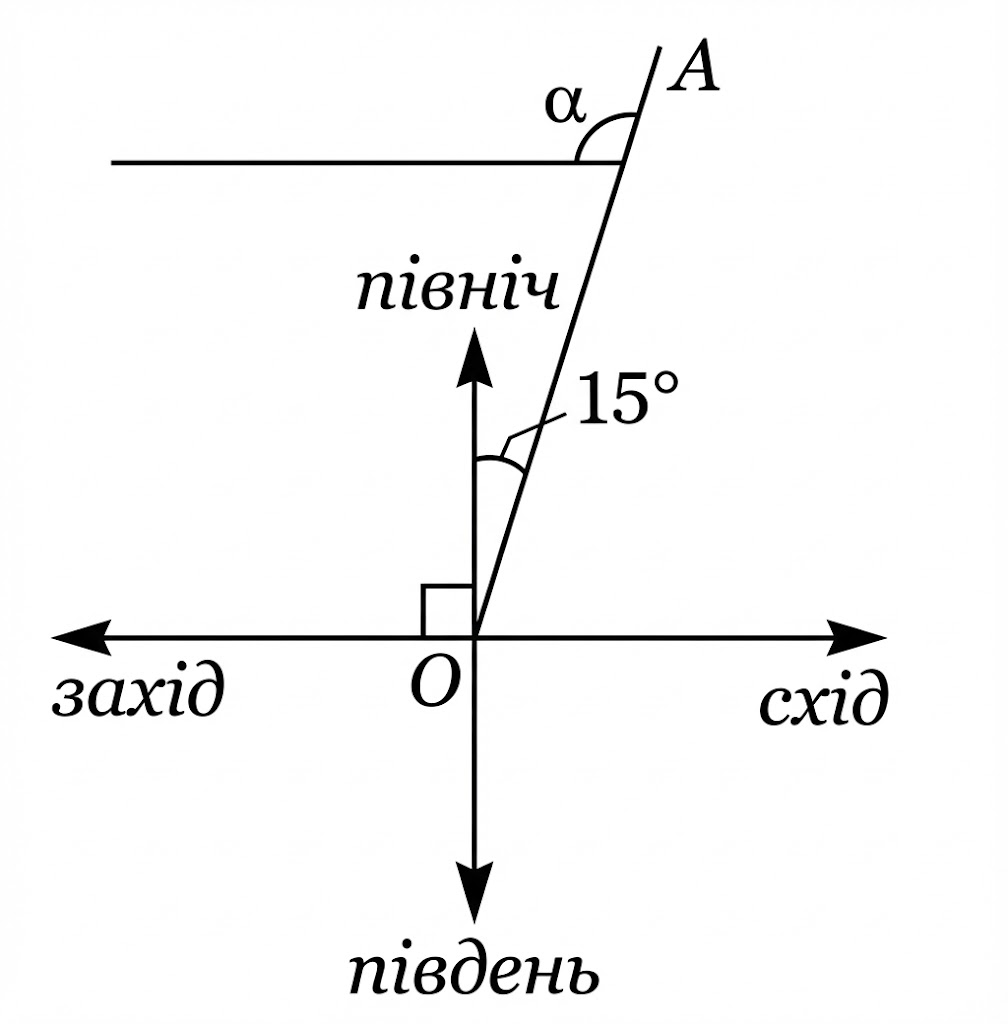
\includegraphics[scale=0.15]{tourists_compass.png}
\end{flushright}
\end{minipage}
\par\penalty-20\vspace{0.25cm}
\end{samepage}
\endgroup

\begingroup
% --- макроси, перенесені зі старого файлу теми ---
\providecommand{\matchingLayout}{}\renewcommand{\matchingLayout}[3]{
    \noindent
    \begin{minipage}[t]{0.36\textwidth}\vspace{0pt}\raggedright
       
        #1
    \end{minipage}%
    \hfill
    \begin{minipage}[t]{0.43\textwidth}\vspace{0pt}\raggedright
        
        #2
    \end{minipage}%
    \hfill
    \begin{minipage}[t]{0.19\textwidth}\vspace{0pt}\raggedright
        \vspace{0pt} % Хаки для вирівнювання minipage по верху
        \begin{flushright}
        #3
        \end{flushright}
    \end{minipage}
}

% --- сумісність зі старою базою (діє, якщо тема не має власного визначення) ---
\providecommand{\trigStyle}[1]{#1}
\providecommand{\answerTableSmall}[5]{%
\begingroup\setlength{\tabcolsep}{2pt}\small\nmtSetCell
\begin{tabular}{|*{5}{>{\centering\arraybackslash}m{\nmtcellw}|}}
\hline
\rule[-0.2cm]{0pt}{0.6cm}\textbf{А} & \textbf{Б} & \textbf{В} & \textbf{Г} & \textbf{Д} \\
\hline
\rule[-0.4cm]{0pt}{0.9cm}#1 & \rule[-0.4cm]{0pt}{0.9cm}#2 & \rule[-0.4cm]{0pt}{0.9cm}#3 & \rule[-0.4cm]{0pt}{0.9cm}#4 & \rule[-0.4cm]{0pt}{0.9cm}#5 \\
\hline
\end{tabular}\endgroup}
\providecommand{\matchingLayout}[3]{%
    \noindent
    \begin{minipage}[t]{0.36\textwidth}\vspace{0pt}\raggedright
        #1
    \end{minipage}%
    \hfill
    \begin{minipage}[t]{0.43\textwidth}\vspace{0pt}\raggedright
        #2
    \end{minipage}%
    \hfill
    \begin{minipage}[t]{0.19\textwidth}
        \vspace{0pt}
        \begin{flushright}
        #3
        \end{flushright}
    \end{minipage}}
\providecommand{\matchingLayoutBottom}[2]{%
    \noindent
    \begin{minipage}[t]{0.48\textwidth}\vspace{0pt}\raggedright
        #1
    \end{minipage}%
    \hfill
    \begin{minipage}[t]{0.48\textwidth}\vspace{0pt}\raggedright
        #2
    \end{minipage}
    \vspace{0.5cm}
    \noindent
    \matchingGrid}
\providecommand{\answerListVertical}[5]{%
    \par\nopagebreak\vspace{0.2cm}
    \begin{itemize}[itemsep=0.4cm, leftmargin=1.5cm, labelsep=0.5cm]
        \item[\textbf{А}] #1
        \item[\textbf{Б}] #2
        \item[\textbf{В}] #3
        \item[\textbf{Г}] #4
        \item[\textbf{Д}] #5
    \end{itemize}
    \vspace{0.2cm}}
\begin{samepage}
\noindent\zadnum Розв'яжіть систему нерівностей $\begin{cases} x^2 + 9 \geqslant 0, \\ 2^x > \displaystyle\frac{1}{16}. \end{cases}$

\nmtnobreak
\answerTable{$[-3; +\infty)$}{$(-4; +\infty)$}{$(-4; -3]$}{$(-4; -3] \cup [3; +\infty)$}{$\varnothing$}
\par\penalty-20
\end{samepage}
\endgroup

\begin{samepage}
\zadtask{Скільки всього ребер має шестикутна піраміда?}
\answerTable{$6$}{$7$}{$12$}{$14$}{$18$}
\par\penalty-20
\end{samepage}

\begingroup
% --- сумісність зі старою базою (діє, якщо тема не має власного визначення) ---
\providecommand{\trigStyle}[1]{#1}
\providecommand{\answerTableSmall}[5]{%
\begingroup\setlength{\tabcolsep}{2pt}\small\nmtSetCell
\begin{tabular}{|*{5}{>{\centering\arraybackslash}m{\nmtcellw}|}}
\hline
\rule[-0.2cm]{0pt}{0.6cm}\textbf{А} & \textbf{Б} & \textbf{В} & \textbf{Г} & \textbf{Д} \\
\hline
\rule[-0.4cm]{0pt}{0.9cm}#1 & \rule[-0.4cm]{0pt}{0.9cm}#2 & \rule[-0.4cm]{0pt}{0.9cm}#3 & \rule[-0.4cm]{0pt}{0.9cm}#4 & \rule[-0.4cm]{0pt}{0.9cm}#5 \\
\hline
\end{tabular}\endgroup}
\providecommand{\matchingLayout}[3]{%
    \noindent
    \begin{minipage}[t]{0.36\textwidth}\vspace{0pt}\raggedright
        #1
    \end{minipage}%
    \hfill
    \begin{minipage}[t]{0.43\textwidth}\vspace{0pt}\raggedright
        #2
    \end{minipage}%
    \hfill
    \begin{minipage}[t]{0.19\textwidth}
        \vspace{0pt}
        \begin{flushright}
        #3
        \end{flushright}
    \end{minipage}}
\providecommand{\matchingLayoutBottom}[2]{%
    \noindent
    \begin{minipage}[t]{0.48\textwidth}\vspace{0pt}\raggedright
        #1
    \end{minipage}%
    \hfill
    \begin{minipage}[t]{0.48\textwidth}\vspace{0pt}\raggedright
        #2
    \end{minipage}
    \vspace{0.5cm}
    \noindent
    \matchingGrid}
\providecommand{\answerListVertical}[5]{%
    \par\nopagebreak\vspace{0.2cm}
    \begin{itemize}[itemsep=0.4cm, leftmargin=1.5cm, labelsep=0.5cm]
        \item[\textbf{А}] #1
        \item[\textbf{Б}] #2
        \item[\textbf{В}] #3
        \item[\textbf{Г}] #4
        \item[\textbf{Д}] #5
    \end{itemize}
    \vspace{0.2cm}}
\begin{samepage}
\zadtask{Укажіть проміжок, якому належить значення виразу $\sqrt{5} \cdot \sqrt{6}$.}
\answerTable{$(4; 6]$}{$(2; 4]$}{$(0; 2]$}{$(8; 10]$}{$(6; 8]$}
\par\penalty-20
\end{samepage}
\endgroup

\begin{samepage}
\zadtask{Якому проміжку належить корінь рівняння $2^{x}\cdot 50^{x} = 0{,}0001$?}
\answerTable{$(-\infty;\, -4)$}{$[-4;\, -2)$}{$[-2;\, -1)$}{$[-1;\, 0)$}{$[0;\, +\infty)$}
\par\penalty-20
\end{samepage}

\begingroup
% --- макроси, перенесені зі старого файлу теми ---
\providecommand{\matchingLayout}{}\renewcommand{\matchingLayout}[3]{
    \noindent
    \begin{minipage}[t]{0.36\textwidth}\vspace{0pt}\raggedright
       
        #1
    \end{minipage}%
    \hfill
    \begin{minipage}[t]{0.43\textwidth}\vspace{0pt}\raggedright
        
        #2
    \end{minipage}%
    \hfill
    \begin{minipage}[t]{0.19\textwidth}\vspace{0pt}\raggedright
        \vspace{0pt} % Хаки для вирівнювання minipage по верху
        \begin{flushright}
        #3
        \end{flushright}
    \end{minipage}
}

% --- макроси з файлів сесій НМТ-2026 (для рисунків) ---
\renewcommand{\headrulewidth}{0.4pt}
\renewcommand{\footrulewidth}{0.4pt}

% --- сумісність зі старою базою (діє, якщо тема не має власного визначення) ---
\providecommand{\trigStyle}[1]{#1}
\providecommand{\answerTableSmall}[5]{%
\begingroup\setlength{\tabcolsep}{2pt}\small\nmtSetCell
\begin{tabular}{|*{5}{>{\centering\arraybackslash}m{\nmtcellw}|}}
\hline
\rule[-0.2cm]{0pt}{0.6cm}\textbf{А} & \textbf{Б} & \textbf{В} & \textbf{Г} & \textbf{Д} \\
\hline
\rule[-0.4cm]{0pt}{0.9cm}#1 & \rule[-0.4cm]{0pt}{0.9cm}#2 & \rule[-0.4cm]{0pt}{0.9cm}#3 & \rule[-0.4cm]{0pt}{0.9cm}#4 & \rule[-0.4cm]{0pt}{0.9cm}#5 \\
\hline
\end{tabular}\endgroup}
\providecommand{\matchingLayout}[3]{%
    \noindent
    \begin{minipage}[t]{0.36\textwidth}\vspace{0pt}\raggedright
        #1
    \end{minipage}%
    \hfill
    \begin{minipage}[t]{0.43\textwidth}\vspace{0pt}\raggedright
        #2
    \end{minipage}%
    \hfill
    \begin{minipage}[t]{0.19\textwidth}
        \vspace{0pt}
        \begin{flushright}
        #3
        \end{flushright}
    \end{minipage}}
\providecommand{\matchingLayoutBottom}[2]{%
    \noindent
    \begin{minipage}[t]{0.48\textwidth}\vspace{0pt}\raggedright
        #1
    \end{minipage}%
    \hfill
    \begin{minipage}[t]{0.48\textwidth}\vspace{0pt}\raggedright
        #2
    \end{minipage}
    \vspace{0.5cm}
    \noindent
    \matchingGrid}
\providecommand{\answerListVertical}[5]{%
    \par\nopagebreak\vspace{0.2cm}
    \begin{itemize}[itemsep=0.4cm, leftmargin=1.5cm, labelsep=0.5cm]
        \item[\textbf{А}] #1
        \item[\textbf{Б}] #2
        \item[\textbf{В}] #3
        \item[\textbf{Г}] #4
        \item[\textbf{Д}] #5
    \end{itemize}
    \vspace{0.2cm}}
\begin{samepage}
\noindent\zadnum Укажіть із-поміж наведених рисунок, на якому \textit{може} бути зображено графік функції $y = kx + b$, якщо $k = 0$.

\nmtnobreak
\nopagebreak\nbvspace{0.3cm}
\begin{center}
\begingroup
\setlength{\tabcolsep}{2pt}
\begin{tabular}{|*{5}{>{\centering\arraybackslash}m{3.0cm}|}}
\hline
\rule[-0.2cm]{0pt}{0.6cm}\textbf{А} & \textbf{Б} & \textbf{В} & \textbf{Г} & \textbf{Д} \\
\hline
\begin{nmtfit}\begin{tikzpicture}[scale=0.45, baseline={(0,0)}]
    \draw[->, >=stealth] (-2.5,0) -- (2.5,0) node[below] {$x$};
    \draw[->, >=stealth] (0,-2.5) -- (0,2.5) node[left] {$y$};
    \node[below left] at (0,0) {\tiny $0$};
    %
    \draw[thick] (-1,2.5) -- (1,-2.5);
\end{tikzpicture}\end{nmtfit} &
\begin{nmtfit}\begin{tikzpicture}[scale=0.45, baseline={(0,0)}]
    \draw[->, >=stealth] (-2.5,0) -- (2.5,0) node[below] {$x$};
    \draw[->, >=stealth] (0,-2.5) -- (0,2.5) node[left] {$y$};
    \node[below left] at (0,0) {\tiny $0$};
    %
    \draw[thick] (-2.5,1) -- (2.5,1);
\end{tikzpicture}\end{nmtfit} &
\begin{nmtfit}\begin{tikzpicture}[scale=0.45, baseline={(0,0)}]
    \draw[->, >=stealth] (-2.5,0) -- (2.5,0) node[below] {$x$};
    \draw[->, >=stealth] (0,-2.5) -- (0,2.5) node[left] {$y$};
    \node[below right] at (0,0) {\tiny $0$};
    %
    \draw[thick] (-2,-2) -- (2,2);
\end{tikzpicture}\end{nmtfit} &
\begin{nmtfit}\begin{tikzpicture}[scale=0.45, baseline={(0,0)}]
    \draw[->, >=stealth] (-2.5,0) -- (2.5,0) node[below] {$x$};
    \draw[->, >=stealth] (0,-2.5) -- (0,2.5) node[left] {$y$};
    \node[below left] at (0,0) {\tiny $0$};
    %
    \draw[thick] (1,-2.5) -- (1,2.5);
\end{tikzpicture}\end{nmtfit} &
\begin{nmtfit}\begin{tikzpicture}[scale=0.45, baseline={(0,0)}]
    \draw[->, >=stealth] (-2.5,0) -- (2.5,0) node[below] {$x$};
    \draw[->, >=stealth] (0,-2.5) -- (0,2.5) node[left] {$y$};
    \node[below left] at (0,0) {\tiny $0$};
    %
    \draw[thick] (-2,2) -- (2,-2);
\end{tikzpicture}\end{nmtfit} \\
\hline
\end{tabular}
\endgroup
\end{center}
\par\penalty-20\vspace{0.25cm}
\end{samepage}
\endgroup

\begingroup
% --- макроси з файлів сесій НМТ-2026 (для рисунків) ---
\renewcommand{\headrulewidth}{0.4pt}
\renewcommand{\footrulewidth}{0.4pt}
\definecolor{gold}{RGB}{240, 190, 40}
\definecolor{silver}{RGB}{170, 170, 175}
\definecolor{bronze}{RGB}{190, 120, 70}
\definecolor{hexcol}{RGB}{200,110,60}
\providecommand{\hexthree}{}\renewcommand{\hexthree}[2]{%
    \draw[hexcol, line width=1.1pt]
        ($(#1,#2)+(0:30)$) -- ($(#1,#2)+(60:30)$) -- ($(#1,#2)+(120:30)$) --
        ($(#1,#2)+(180:30)$) -- ($(#1,#2)+(240:30)$) -- ($(#1,#2)+(300:30)$) -- cycle;
}

% --- сумісність зі старою базою (діє, якщо тема не має власного визначення) ---
\providecommand{\trigStyle}[1]{#1}
\providecommand{\answerTableSmall}[5]{%
\begingroup\setlength{\tabcolsep}{2pt}\small\nmtSetCell
\begin{tabular}{|*{5}{>{\centering\arraybackslash}m{\nmtcellw}|}}
\hline
\rule[-0.2cm]{0pt}{0.6cm}\textbf{А} & \textbf{Б} & \textbf{В} & \textbf{Г} & \textbf{Д} \\
\hline
\rule[-0.4cm]{0pt}{0.9cm}#1 & \rule[-0.4cm]{0pt}{0.9cm}#2 & \rule[-0.4cm]{0pt}{0.9cm}#3 & \rule[-0.4cm]{0pt}{0.9cm}#4 & \rule[-0.4cm]{0pt}{0.9cm}#5 \\
\hline
\end{tabular}\endgroup}
\providecommand{\matchingLayout}[3]{%
    \noindent
    \begin{minipage}[t]{0.36\textwidth}\vspace{0pt}\raggedright
        #1
    \end{minipage}%
    \hfill
    \begin{minipage}[t]{0.43\textwidth}\vspace{0pt}\raggedright
        #2
    \end{minipage}%
    \hfill
    \begin{minipage}[t]{0.19\textwidth}
        \vspace{0pt}
        \begin{flushright}
        #3
        \end{flushright}
    \end{minipage}}
\providecommand{\matchingLayoutBottom}[2]{%
    \noindent
    \begin{minipage}[t]{0.48\textwidth}\vspace{0pt}\raggedright
        #1
    \end{minipage}%
    \hfill
    \begin{minipage}[t]{0.48\textwidth}\vspace{0pt}\raggedright
        #2
    \end{minipage}
    \vspace{0.5cm}
    \noindent
    \matchingGrid}
\providecommand{\answerListVertical}[5]{%
    \par\nopagebreak\vspace{0.2cm}
    \begin{itemize}[itemsep=0.4cm, leftmargin=1.5cm, labelsep=0.5cm]
        \item[\textbf{А}] #1
        \item[\textbf{Б}] #2
        \item[\textbf{В}] #3
        \item[\textbf{Г}] #4
        \item[\textbf{Д}] #5
    \end{itemize}
    \vspace{0.2cm}}
\begin{samepage}
\zadtask{Задано довільний трикутник $ABC$, у якому $AM$~--- медіана. Які з наведених тверджень є правильними?}

\nmtnobreak
\nopagebreak\nbvspace{0.2cm}
\begin{tabular}{r@{\hspace{0.5em}}p{14cm}}
I. & $BM = MC$. \\
II. & $\angle BAM = \angle MAC$. \\
III. & Площа трикутника $ABM$ дорівнює площі трикутника $MCA$. \\
\end{tabular}

\nmtnobreak
\answerTable{лише I та III}{лише I}{лише III}{лише II та III}{I, II та III}
\par\penalty-20
\end{samepage}
\endgroup

\begingroup
% --- макроси з файлів сесій НМТ-2026 (для рисунків) ---
\renewcommand{\headrulewidth}{0.4pt}
\renewcommand{\footrulewidth}{0.4pt}

% --- сумісність зі старою базою (діє, якщо тема не має власного визначення) ---
\providecommand{\trigStyle}[1]{#1}
\providecommand{\answerTableSmall}[5]{%
\begingroup\setlength{\tabcolsep}{2pt}\small\nmtSetCell
\begin{tabular}{|*{5}{>{\centering\arraybackslash}m{\nmtcellw}|}}
\hline
\rule[-0.2cm]{0pt}{0.6cm}\textbf{А} & \textbf{Б} & \textbf{В} & \textbf{Г} & \textbf{Д} \\
\hline
\rule[-0.4cm]{0pt}{0.9cm}#1 & \rule[-0.4cm]{0pt}{0.9cm}#2 & \rule[-0.4cm]{0pt}{0.9cm}#3 & \rule[-0.4cm]{0pt}{0.9cm}#4 & \rule[-0.4cm]{0pt}{0.9cm}#5 \\
\hline
\end{tabular}\endgroup}
\providecommand{\matchingLayout}[3]{%
    \noindent
    \begin{minipage}[t]{0.36\textwidth}\vspace{0pt}\raggedright
        #1
    \end{minipage}%
    \hfill
    \begin{minipage}[t]{0.43\textwidth}\vspace{0pt}\raggedright
        #2
    \end{minipage}%
    \hfill
    \begin{minipage}[t]{0.19\textwidth}
        \vspace{0pt}
        \begin{flushright}
        #3
        \end{flushright}
    \end{minipage}}
\providecommand{\matchingLayoutBottom}[2]{%
    \noindent
    \begin{minipage}[t]{0.48\textwidth}\vspace{0pt}\raggedright
        #1
    \end{minipage}%
    \hfill
    \begin{minipage}[t]{0.48\textwidth}\vspace{0pt}\raggedright
        #2
    \end{minipage}
    \vspace{0.5cm}
    \noindent
    \matchingGrid}
\providecommand{\answerListVertical}[5]{%
    \par\nopagebreak\vspace{0.2cm}
    \begin{itemize}[itemsep=0.4cm, leftmargin=1.5cm, labelsep=0.5cm]
        \item[\textbf{А}] #1
        \item[\textbf{Б}] #2
        \item[\textbf{В}] #3
        \item[\textbf{Г}] #4
        \item[\textbf{Д}] #5
    \end{itemize}
    \vspace{0.2cm}}
\begin{samepage}
\noindent\zadnum Обчисліть $\displaystyle\int\limits_0^{\pi} 2\sin x \, dx$.

\nmtnobreak
\nopagebreak\nbvspace{0.3cm}
\answerTable{$0$}{$2$}{$4$}{$-2$}{$-4$}
\par\penalty-20
\end{samepage}
\endgroup

\begingroup
% --- макроси з файлів сесій НМТ-2026 (для рисунків) ---
\renewcommand{\headrulewidth}{0.4pt}
\renewcommand{\footrulewidth}{0.4pt}
\definecolor{gold}{RGB}{240, 190, 40}
\definecolor{silver}{RGB}{170, 170, 175}
\definecolor{bronze}{RGB}{190, 120, 70}

% --- сумісність зі старою базою (діє, якщо тема не має власного визначення) ---
\providecommand{\trigStyle}[1]{#1}
\providecommand{\answerTableSmall}[5]{%
\begingroup\setlength{\tabcolsep}{2pt}\small\nmtSetCell
\begin{tabular}{|*{5}{>{\centering\arraybackslash}m{\nmtcellw}|}}
\hline
\rule[-0.2cm]{0pt}{0.6cm}\textbf{А} & \textbf{Б} & \textbf{В} & \textbf{Г} & \textbf{Д} \\
\hline
\rule[-0.4cm]{0pt}{0.9cm}#1 & \rule[-0.4cm]{0pt}{0.9cm}#2 & \rule[-0.4cm]{0pt}{0.9cm}#3 & \rule[-0.4cm]{0pt}{0.9cm}#4 & \rule[-0.4cm]{0pt}{0.9cm}#5 \\
\hline
\end{tabular}\endgroup}
\providecommand{\matchingLayout}[3]{%
    \noindent
    \begin{minipage}[t]{0.36\textwidth}\vspace{0pt}\raggedright
        #1
    \end{minipage}%
    \hfill
    \begin{minipage}[t]{0.43\textwidth}\vspace{0pt}\raggedright
        #2
    \end{minipage}%
    \hfill
    \begin{minipage}[t]{0.19\textwidth}
        \vspace{0pt}
        \begin{flushright}
        #3
        \end{flushright}
    \end{minipage}}
\providecommand{\matchingLayoutBottom}[2]{%
    \noindent
    \begin{minipage}[t]{0.48\textwidth}\vspace{0pt}\raggedright
        #1
    \end{minipage}%
    \hfill
    \begin{minipage}[t]{0.48\textwidth}\vspace{0pt}\raggedright
        #2
    \end{minipage}
    \vspace{0.5cm}
    \noindent
    \matchingGrid}
\providecommand{\answerListVertical}[5]{%
    \par\nopagebreak\vspace{0.2cm}
    \begin{itemize}[itemsep=0.4cm, leftmargin=1.5cm, labelsep=0.5cm]
        \item[\textbf{А}] #1
        \item[\textbf{Б}] #2
        \item[\textbf{В}] #3
        \item[\textbf{Г}] #4
        \item[\textbf{Д}] #5
    \end{itemize}
    \vspace{0.2cm}}
\begin{samepage}
\noindent\zadnum \begin{minipage}[t]{0.55\textwidth}
На дитячій каруселі розташовано 19 транспортних засобів: човники, літачки й машинки (див. рисунок). Дмитрик навмання сідає в один із транспортних засобів, \textit{окрім літачків}. Яка \textbf{ймовірність} того, що він сяде в \textit{машинку}?
\end{minipage}
\hfill
\begin{minipage}[t]{0.40\textwidth}
\nopagebreak\nbvspace{-0.3cm}
\begin{center}
\begin{nmtfit}\begin{tikzpicture}[scale=0.8]
    %
    \fill[yellow!10] (0,0) circle (4.0cm);
    \fill[cyan!10] (0,0) circle (3.2cm); %
    \fill[green!5] (0,0) circle (2.0cm); 

    %
    \draw[thick, gray!40] (0,0) circle (4.0cm);
    \draw[thick, gray!40] (0,0) circle (3.2cm);
    \draw[thick, gray!40] (0,0) circle (2.0cm);

    %
    \tikzset{icon/.style={thick, line join=round}}

    %
    \foreach \i in {1,...,10} {
        \pgfmathsetmacro{\ang}{\i * 360/10}
        \begin{scope}[rotate=\ang, shift={(3.5,0)}]
            \begin{scope}[rotate=90]
                 \draw[icon, fill=brown!80!black] (-0.35,0) arc (180:360:0.35 and 0.25) -- cycle;
                 \draw[icon, fill=white] (0,0.05) -- (0.25,0.05) -- (0,0.3) -- cycle; 
            \end{scope}
        \end{scope}
    }

    %
    \foreach \i in {1,...,5} {
        \pgfmathsetmacro{\ang}{\i * 360/5}
        \begin{scope}[rotate=\ang, shift={(2.6,0)}]
            \begin{scope}[rotate=90]
                \draw[icon, fill=cyan!80!blue] (-0.35,-0.2) rectangle (0.35,0.2);
                \draw[icon, fill=black] (-0.25,-0.2) circle (0.1); %
                \draw[icon, fill=black] (0.25,-0.2) circle (0.1);
                \draw[icon, fill=cyan!30] (-0.2,0) -- (-0.2,0.15) -- (0.2,0.15) -- (0.2,0) -- cycle; %
            \end{scope}
        \end{scope}
    }

    %
    \foreach \i in {1,...,4} {
        \pgfmathsetmacro{\ang}{\i * 360/4 + 45}
        \begin{scope}[rotate=\ang, shift={(1.2,0)}]
            \begin{scope}[rotate=90] 
                \draw[icon, fill=green!60!black] (0,-0.35) -- (0,0.4); %
                \draw[icon, fill=green!60!black] (-0.35,0) -- (0.35,0); %
                \draw[icon, fill=red] (-0.15,-0.3) -- (0.15,-0.3); %
            \end{scope}
        \end{scope}
    }

    %
    \node[anchor=west, font=\tiny] at (2.9, 3.5) {\textcolor{brown!80!black}{\rule{8pt}{8pt}} човник};
    \node[anchor=west, font=\tiny] at (2.9, 3.0) {\textcolor{green!60!black}{\rule{8pt}{8pt}} літачок};
    \node[anchor=west, font=\tiny] at (2.9, 2.5) {\textcolor{cyan!80!blue}{\rule{8pt}{8pt}} машинка};

\end{tikzpicture}\end{nmtfit}
\end{center}
\end{minipage}

\nmtnobreak
\nopagebreak\nbvspace{0.3cm}
\answerTableTall{$\dfrac{5}{19}$}{$\dfrac{1}{3}$}{$\dfrac{1}{15}$}{$\dfrac{2}{3}$}{$\dfrac{1}{5}$}
\par\penalty-20
\end{samepage}
\endgroup

\begingroup
% --- макроси, перенесені зі старого файлу теми ---
\providecommand{\matchingLayout}{}\renewcommand{\matchingLayout}[3]{
    \noindent
    \begin{minipage}[t]{0.36\textwidth}\vspace{0pt}\raggedright
        #1
    \end{minipage}%
    \hfill
    \begin{minipage}[t]{0.43\textwidth}\vspace{0pt}\raggedright
        #2
    \end{minipage}%
    \hfill
    \begin{minipage}[t]{0.19\textwidth}\vspace{0pt}\raggedright
        \vspace{0pt} 
        \begin{flushright}
        #3
        \end{flushright}
    \end{minipage}
}

% --- макроси з файлів сесій НМТ-2026 (для рисунків) ---
\renewcommand{\headrulewidth}{0.4pt}
\renewcommand{\footrulewidth}{0.4pt}
\definecolor{gold}{RGB}{240, 190, 40}
\definecolor{silver}{RGB}{170, 170, 175}
\definecolor{bronze}{RGB}{190, 120, 70}

% --- сумісність зі старою базою (діє, якщо тема не має власного визначення) ---
\providecommand{\trigStyle}[1]{#1}
\providecommand{\answerTableSmall}[5]{%
\begingroup\setlength{\tabcolsep}{2pt}\small\nmtSetCell
\begin{tabular}{|*{5}{>{\centering\arraybackslash}m{\nmtcellw}|}}
\hline
\rule[-0.2cm]{0pt}{0.6cm}\textbf{А} & \textbf{Б} & \textbf{В} & \textbf{Г} & \textbf{Д} \\
\hline
\rule[-0.4cm]{0pt}{0.9cm}#1 & \rule[-0.4cm]{0pt}{0.9cm}#2 & \rule[-0.4cm]{0pt}{0.9cm}#3 & \rule[-0.4cm]{0pt}{0.9cm}#4 & \rule[-0.4cm]{0pt}{0.9cm}#5 \\
\hline
\end{tabular}\endgroup}
\providecommand{\matchingLayout}[3]{%
    \noindent
    \begin{minipage}[t]{0.36\textwidth}\vspace{0pt}\raggedright
        #1
    \end{minipage}%
    \hfill
    \begin{minipage}[t]{0.43\textwidth}\vspace{0pt}\raggedright
        #2
    \end{minipage}%
    \hfill
    \begin{minipage}[t]{0.19\textwidth}
        \vspace{0pt}
        \begin{flushright}
        #3
        \end{flushright}
    \end{minipage}}
\providecommand{\matchingLayoutBottom}[2]{%
    \noindent
    \begin{minipage}[t]{0.48\textwidth}\vspace{0pt}\raggedright
        #1
    \end{minipage}%
    \hfill
    \begin{minipage}[t]{0.48\textwidth}\vspace{0pt}\raggedright
        #2
    \end{minipage}
    \vspace{0.5cm}
    \noindent
    \matchingGrid}
\providecommand{\answerListVertical}[5]{%
    \par\nopagebreak\vspace{0.2cm}
    \begin{itemize}[itemsep=0.4cm, leftmargin=1.5cm, labelsep=0.5cm]
        \item[\textbf{А}] #1
        \item[\textbf{Б}] #2
        \item[\textbf{В}] #3
        \item[\textbf{Г}] #4
        \item[\textbf{Д}] #5
    \end{itemize}
    \vspace{0.2cm}}
\begin{samepage}
\noindent
\begin{minipage}[c]{0.58\textwidth}
\zadnum У прямокутній системі координат $xy$ зображено квадрат $KLMN$, $K(-1; 0)$, $L(-1; 2)$, $M(1; 2)$, $N(1; 0)$ (див. рисунок). Скільки спільних точок з квадратом $KLMN$ має графік рівняння $x^2 + y^2 = 4$?
\end{minipage}%
\hfill
\begin{minipage}[c]{0.40\textwidth}
\centering
\begin{nmtfit}\begin{tikzpicture}[scale=0.85, thick]
    \draw[step=1cm, gray!40, thin] (-2,-1) grid (2,3);
    \draw[->] (-2.3,0) -- (2.3,0) node[right] {$x$};
    \draw[->] (0,-1.3) -- (0,3.3) node[above] {$y$};
    \node[below right, font=\scriptsize] at (0,0) {$0$};
    \node[below, font=\scriptsize] at (-1,0) {$-1$};
    \node[below right, font=\scriptsize] at (1,0) {$1$};
    \node[above left, font=\scriptsize] at (0,1) {$1$};
    \node[above left, font=\scriptsize] at (0,2) {$2$};
    \draw[mainGreen, very thick] (-1,0) rectangle (1,2);
    \node[below left, font=\scriptsize] at (-1,0) {$K$};
    \node[above left, font=\scriptsize] at (-1,2) {$L$};
    \node[above right, font=\scriptsize] at (1,2) {$M$};
    \node[below right, font=\scriptsize] at (1,0) {$N$};

\end{tikzpicture}\end{nmtfit}
\end{minipage}
\par\nbvspace{0.2cm}
\answerTable{жодної}{лише одну}{лише дві}{лише три}{більше трьох}
\par\penalty-20
\end{samepage}
\endgroup

\begingroup
% --- макроси, перенесені зі старого файлу теми ---
\providecommand{\matchingLayout}{}\renewcommand{\matchingLayout}[3]{
    \noindent
    \begin{minipage}[t]{0.36\textwidth}\vspace{0pt}\raggedright
       
        #1
    \end{minipage}%
    \hfill
    \begin{minipage}[t]{0.43\textwidth}\vspace{0pt}\raggedright
        
        #2
    \end{minipage}%
    \hfill
    \begin{minipage}[t]{0.19\textwidth}\vspace{0pt}\raggedright
        \vspace{0pt} % Хаки для вирівнювання minipage по верху
        \begin{flushright}
        #3
        \end{flushright}
    \end{minipage}
}
\providecommand{\trigStyle}{}\renewcommand{\trigStyle}[1]{\textbf{#1}}

% --- сумісність зі старою базою (діє, якщо тема не має власного визначення) ---
\providecommand{\trigStyle}[1]{#1}
\providecommand{\answerTableSmall}[5]{%
\begingroup\setlength{\tabcolsep}{2pt}\small\nmtSetCell
\begin{tabular}{|*{5}{>{\centering\arraybackslash}m{\nmtcellw}|}}
\hline
\rule[-0.2cm]{0pt}{0.6cm}\textbf{А} & \textbf{Б} & \textbf{В} & \textbf{Г} & \textbf{Д} \\
\hline
\rule[-0.4cm]{0pt}{0.9cm}#1 & \rule[-0.4cm]{0pt}{0.9cm}#2 & \rule[-0.4cm]{0pt}{0.9cm}#3 & \rule[-0.4cm]{0pt}{0.9cm}#4 & \rule[-0.4cm]{0pt}{0.9cm}#5 \\
\hline
\end{tabular}\endgroup}
\providecommand{\matchingLayout}[3]{%
    \noindent
    \begin{minipage}[t]{0.36\textwidth}\vspace{0pt}\raggedright
        #1
    \end{minipage}%
    \hfill
    \begin{minipage}[t]{0.43\textwidth}\vspace{0pt}\raggedright
        #2
    \end{minipage}%
    \hfill
    \begin{minipage}[t]{0.19\textwidth}
        \vspace{0pt}
        \begin{flushright}
        #3
        \end{flushright}
    \end{minipage}}
\providecommand{\matchingLayoutBottom}[2]{%
    \noindent
    \begin{minipage}[t]{0.48\textwidth}\vspace{0pt}\raggedright
        #1
    \end{minipage}%
    \hfill
    \begin{minipage}[t]{0.48\textwidth}\vspace{0pt}\raggedright
        #2
    \end{minipage}
    \vspace{0.5cm}
    \noindent
    \matchingGrid}
\providecommand{\answerListVertical}[5]{%
    \par\nopagebreak\vspace{0.2cm}
    \begin{itemize}[itemsep=0.4cm, leftmargin=1.5cm, labelsep=0.5cm]
        \item[\textbf{А}] #1
        \item[\textbf{Б}] #2
        \item[\textbf{В}] #3
        \item[\textbf{Г}] #4
        \item[\textbf{Д}] #5
    \end{itemize}
    \vspace{0.2cm}}
\begin{samepage}
\zadtask{Спростіть вираз $\dfrac{1 - \cos^2 \alpha}{\operatorname{tg} \alpha \cdot \cos \alpha}$.}
\answerTable{$\sin \alpha$}{$\operatorname{tg} \alpha$}{$1$}{$\cos \alpha$}{$0$}
\par\penalty-20
\end{samepage}
\endgroup

\begin{samepage}
\noindent
\begin{minipage}[c]{0.58\textwidth}
\zadnum Колесо має $10$ спиць, розміщених рівномірно: кути між будь-якими двома сусідніми спицями рівні (див. рисунок). Визначте градусну міру кута $\alpha$.
\end{minipage}
\hfill
\begin{minipage}[c]{0.40\textwidth}
\centering
\begin{nmtfit}\begin{tikzpicture}[scale=1.0, thick]
    \coordinate (O) at (0,0);
    \draw[mainGreen!80!black] (O) circle (2);
    \foreach \a in {18,54,...,342} {
        \draw[mainGreen!80!black] (O) -- (\a:2);
    }
    \coordinate (P1) at (18:2);
    \coordinate (P2) at (126:2);
    \pic[draw=yearOrange, line width=0.8pt, "$\alpha$", angle radius=0.6cm,
         angle eccentricity=1.6, font=\small] {angle = P1--O--P2};
    \fill (O) circle (1.5pt);
\end{tikzpicture}\end{nmtfit}
\end{minipage}
\par\nbvspace{0.2cm}
\answerTable{$18^\circ$}{$36^\circ$}{$54^\circ$}{$72^\circ$}{$108^\circ$}
\par\penalty-20
\end{samepage}

\begingroup
% --- сумісність зі старою базою (діє, якщо тема не має власного визначення) ---
\providecommand{\trigStyle}[1]{#1}
\providecommand{\answerTableSmall}[5]{%
\begingroup\setlength{\tabcolsep}{2pt}\small\nmtSetCell
\begin{tabular}{|*{5}{>{\centering\arraybackslash}m{\nmtcellw}|}}
\hline
\rule[-0.2cm]{0pt}{0.6cm}\textbf{А} & \textbf{Б} & \textbf{В} & \textbf{Г} & \textbf{Д} \\
\hline
\rule[-0.4cm]{0pt}{0.9cm}#1 & \rule[-0.4cm]{0pt}{0.9cm}#2 & \rule[-0.4cm]{0pt}{0.9cm}#3 & \rule[-0.4cm]{0pt}{0.9cm}#4 & \rule[-0.4cm]{0pt}{0.9cm}#5 \\
\hline
\end{tabular}\endgroup}
\providecommand{\matchingLayout}[3]{%
    \noindent
    \begin{minipage}[t]{0.36\textwidth}\vspace{0pt}\raggedright
        #1
    \end{minipage}%
    \hfill
    \begin{minipage}[t]{0.43\textwidth}\vspace{0pt}\raggedright
        #2
    \end{minipage}%
    \hfill
    \begin{minipage}[t]{0.19\textwidth}
        \vspace{0pt}
        \begin{flushright}
        #3
        \end{flushright}
    \end{minipage}}
\providecommand{\matchingLayoutBottom}[2]{%
    \noindent
    \begin{minipage}[t]{0.48\textwidth}\vspace{0pt}\raggedright
        #1
    \end{minipage}%
    \hfill
    \begin{minipage}[t]{0.48\textwidth}\vspace{0pt}\raggedright
        #2
    \end{minipage}
    \vspace{0.5cm}
    \noindent
    \matchingGrid}
\providecommand{\answerListVertical}[5]{%
    \par\nopagebreak\vspace{0.2cm}
    \begin{itemize}[itemsep=0.4cm, leftmargin=1.5cm, labelsep=0.5cm]
        \item[\textbf{А}] #1
        \item[\textbf{Б}] #2
        \item[\textbf{В}] #3
        \item[\textbf{Г}] #4
        \item[\textbf{Д}] #5
    \end{itemize}
    \vspace{0.2cm}}
\begin{samepage}
\zadtask{Розв'яжіть систему рівнянь $\begin{cases} \dfrac{x}{2x + y} = \dfrac{1}{5}, \\[0.6cm] 4x + 2 = y. \end{cases}$ Якщо $(x_0; y_0)$ --- розв'язок системи, то $x_0 + y_0 =$}
\answerTable{$12$}{$8$}{$-6$}{$-8$}{$6$}
\par\penalty-20
\end{samepage}
\endgroup

\instructionBox{У завданнях 16--18 до кожного з трьох рядків інформації, позначених цифрами, доберіть один правильний, на Вашу думку, варіант, позначений буквою.}

\begin{samepage}
\zadtask{Установіть відповідність між виразом \mbox{(1--3)} і його значенням \mbox{(А--Д)}, якщо $a = \dfrac{2}{3}$.
\par\nopagebreak\nbvspace{0.3cm}
\noindent
\matchingLayout{
\matchHead{Вираз}
\matchItem{1}{$\sqrt[3]{\dfrac{a^2}{12}}$}
\matchItem{2}{$\log_3 a + \log_3 \dfrac{27}{2}$}
\matchItem{3}{$\cos(\pi a)$}
}{
\matchHead{Значення виразу}
\matchItem{А}{$3$}
\matchItem{Б}{$2$}
\matchItem{В}{$\dfrac{1}{2}$}
\matchItem{Г}{$\dfrac{1}{3}$}
\matchItem{Д}{$-\dfrac{1}{2}$}
}{
\matchingGrid
}}
\par\penalty-20
\end{samepage}

\begingroup
% --- макроси, перенесені зі старого файлу теми ---
\providecommand{\matchingLayout}{}\renewcommand{\matchingLayout}[3]{
    \noindent
    \begin{minipage}[t]{0.36\textwidth}\vspace{0pt}\raggedright
       
        #1
    \end{minipage}%
    \hfill
    \begin{minipage}[t]{0.43\textwidth}\vspace{0pt}\raggedright
        
        #2
    \end{minipage}%
    \hfill
    \begin{minipage}[t]{0.19\textwidth}\vspace{0pt}\raggedright
        \vspace{0pt} % Хаки для вирівнювання minipage по верху
        \begin{flushright}
        #3
        \end{flushright}
    \end{minipage}
}

% --- макроси з файлів сесій НМТ-2026 (для рисунків) ---
\renewcommand{\headrulewidth}{0.4pt}
\renewcommand{\footrulewidth}{0.4pt}
\definecolor{gold}{RGB}{240, 190, 40}
\definecolor{silver}{RGB}{170, 170, 175}
\definecolor{bronze}{RGB}{190, 120, 70}
\definecolor{bar1}{RGB}{200, 120, 20}
\definecolor{bar2}{RGB}{255, 220, 0}
\definecolor{bar3}{RGB}{220, 30, 30}
\definecolor{bar4}{RGB}{128, 0, 128}
\definecolor{bar5}{RGB}{0, 160, 220}
\definecolor{bar6}{RGB}{120, 180, 50}
\definecolor{hexcol}{RGB}{200,110,60}
\providecommand{\hexthree}{}\renewcommand{\hexthree}[2]{%
    \draw[hexcol, line width=1.1pt]
        ($(#1,#2)+(0:30)$) -- ($(#1,#2)+(60:30)$) -- ($(#1,#2)+(120:30)$) --
        ($(#1,#2)+(180:30)$) -- ($(#1,#2)+(240:30)$) -- ($(#1,#2)+(300:30)$) -- cycle;
}

% --- сумісність зі старою базою (діє, якщо тема не має власного визначення) ---
\providecommand{\trigStyle}[1]{#1}
\providecommand{\answerTableSmall}[5]{%
\begingroup\setlength{\tabcolsep}{2pt}\small\nmtSetCell
\begin{tabular}{|*{5}{>{\centering\arraybackslash}m{\nmtcellw}|}}
\hline
\rule[-0.2cm]{0pt}{0.6cm}\textbf{А} & \textbf{Б} & \textbf{В} & \textbf{Г} & \textbf{Д} \\
\hline
\rule[-0.4cm]{0pt}{0.9cm}#1 & \rule[-0.4cm]{0pt}{0.9cm}#2 & \rule[-0.4cm]{0pt}{0.9cm}#3 & \rule[-0.4cm]{0pt}{0.9cm}#4 & \rule[-0.4cm]{0pt}{0.9cm}#5 \\
\hline
\end{tabular}\endgroup}
\providecommand{\matchingLayout}[3]{%
    \noindent
    \begin{minipage}[t]{0.36\textwidth}\vspace{0pt}\raggedright
        #1
    \end{minipage}%
    \hfill
    \begin{minipage}[t]{0.43\textwidth}\vspace{0pt}\raggedright
        #2
    \end{minipage}%
    \hfill
    \begin{minipage}[t]{0.19\textwidth}
        \vspace{0pt}
        \begin{flushright}
        #3
        \end{flushright}
    \end{minipage}}
\providecommand{\matchingLayoutBottom}[2]{%
    \noindent
    \begin{minipage}[t]{0.48\textwidth}\vspace{0pt}\raggedright
        #1
    \end{minipage}%
    \hfill
    \begin{minipage}[t]{0.48\textwidth}\vspace{0pt}\raggedright
        #2
    \end{minipage}
    \vspace{0.5cm}
    \noindent
    \matchingGrid}
\providecommand{\answerListVertical}[5]{%
    \par\nopagebreak\vspace{0.2cm}
    \begin{itemize}[itemsep=0.4cm, leftmargin=1.5cm, labelsep=0.5cm]
        \item[\textbf{А}] #1
        \item[\textbf{Б}] #2
        \item[\textbf{В}] #3
        \item[\textbf{Г}] #4
        \item[\textbf{Д}] #5
    \end{itemize}
    \vspace{0.2cm}}
\begin{samepage}
\noindent\zadnum Узгодьте функцію (1–3) із її властивістю (А – Д).

\nmtnobreak
\nopagebreak\nbvspace{0.3cm}

\nmtnobreak
\noindent
\matchingLayout{
\matchHead{Функція}
    \matchItem{1}{$y=7x+4$}
\matchItem{2}{$y=-\dfrac{7}{x}$}
\matchItem{3}{$y=\log_{0{,}1}(x-4)$}
}{
\matchHead{Властивість функції}
    \matchItem{А}{парна}
\matchItem{Б}{непарна}
\matchItem{В}{область визначення функції є проміжок $(0; +\infty)$}
\matchItem{Г}{графік функції перетинає вісь $y$ в точці з ординатою $4$}
\matchItem{Д}{спадає на всій області визначення}
}{
\matchingGrid
}
\par\penalty-20\vspace{0.25cm}
\end{samepage}
\endgroup

\begin{samepage}
\zadtask{На рисунку зображено квадрат $ABCD$ та рівнобедрений прямокутний трикутник $AKD$ (прямий кут при вершині $K$), які мають спільну сторону $AD$. Точки $M$ і $N$~--- середини сторін $BC$ і $AD$ відповідно. Периметр прямокутника $ABMN$ дорівнює $18$. Установіть відповідність між величиною \mbox{(1--3)} та її значенням \mbox{(А--Д)}.
\par\nopagebreak\nbvspace{0.3cm}
\begin{center}
\begin{nmtfit}\begin{tikzpicture}[scale=0.55, thick]
    \coordinate (A) at (0,0);
    \coordinate (B) at (0,6);
    \coordinate (C) at (6,6);
    \coordinate (D) at (6,0);
    \coordinate (K) at (3,-3);
    \coordinate (M) at (3,6);
    \coordinate (N) at (3,0);
    \draw (A) -- (B) -- (C) -- (D) -- cycle;
    \draw (A) -- (K) -- (D);
    \draw (M) -- (N);
    \pic[draw, thin, angle radius=0.25cm] {right angle = A--K--D};
    \fill (M) circle (0.12);
    \fill (N) circle (0.12);
    \node[below left] at (A) {$A$};
    \node[above left] at (B) {$B$};
    \node[above right] at (C) {$C$};
    \node[below right] at (D) {$D$};
    \node[below] at (K) {$K$};
    \node[above] at (M) {$M$};
    \node[above right] at (N) {$N$};
\end{tikzpicture}\end{nmtfit}
\end{center}
\nopagebreak\nbvspace{0.2cm}
\noindent
\matchingLayout{
\matchHead{Величина}
\matchItem{1}{довжина сторони квадрата}
\matchItem{2}{відстань від точки $K$ до прямої $BC$}
\matchItem{3}{довжина відрізка $KC$}
}{
\matchHead{Значення}
\matchItem{А}{$6$}
\matchItem{Б}{$3\sqrt{5}$}
\matchItem{В}{$9$}
\matchItem{Г}{$3\sqrt{10}$}
\matchItem{Д}{$12$}
}{
\matchingGrid
}}
\par\penalty-20
\end{samepage}

\instructionBox{Розв'яжіть завдання 19--22. Одержані числові відповіді запишіть у бланку відповідей. Відповідь записуйте лише десятковим дробом, урахувавши положення коми. Знак «мінус» записуйте перед першою цифрою числа.}

\begingroup
% --- макроси з файлів сесій НМТ-2026 (для рисунків) ---
\renewcommand{\headrulewidth}{0.4pt}
\renewcommand{\footrulewidth}{0.4pt}

% --- сумісність зі старою базою (діє, якщо тема не має власного визначення) ---
\providecommand{\trigStyle}[1]{#1}
\providecommand{\answerTableSmall}[5]{%
\begingroup\setlength{\tabcolsep}{2pt}\small\nmtSetCell
\begin{tabular}{|*{5}{>{\centering\arraybackslash}m{\nmtcellw}|}}
\hline
\rule[-0.2cm]{0pt}{0.6cm}\textbf{А} & \textbf{Б} & \textbf{В} & \textbf{Г} & \textbf{Д} \\
\hline
\rule[-0.4cm]{0pt}{0.9cm}#1 & \rule[-0.4cm]{0pt}{0.9cm}#2 & \rule[-0.4cm]{0pt}{0.9cm}#3 & \rule[-0.4cm]{0pt}{0.9cm}#4 & \rule[-0.4cm]{0pt}{0.9cm}#5 \\
\hline
\end{tabular}\endgroup}
\providecommand{\matchingLayout}[3]{%
    \noindent
    \begin{minipage}[t]{0.36\textwidth}\vspace{0pt}\raggedright
        #1
    \end{minipage}%
    \hfill
    \begin{minipage}[t]{0.43\textwidth}\vspace{0pt}\raggedright
        #2
    \end{minipage}%
    \hfill
    \begin{minipage}[t]{0.19\textwidth}
        \vspace{0pt}
        \begin{flushright}
        #3
        \end{flushright}
    \end{minipage}}
\providecommand{\matchingLayoutBottom}[2]{%
    \noindent
    \begin{minipage}[t]{0.48\textwidth}\vspace{0pt}\raggedright
        #1
    \end{minipage}%
    \hfill
    \begin{minipage}[t]{0.48\textwidth}\vspace{0pt}\raggedright
        #2
    \end{minipage}
    \vspace{0.5cm}
    \noindent
    \matchingGrid}
\providecommand{\answerListVertical}[5]{%
    \par\nopagebreak\vspace{0.2cm}
    \begin{itemize}[itemsep=0.4cm, leftmargin=1.5cm, labelsep=0.5cm]
        \item[\textbf{А}] #1
        \item[\textbf{Б}] #2
        \item[\textbf{В}] #3
        \item[\textbf{Г}] #4
        \item[\textbf{Д}] #5
    \end{itemize}
    \vspace{0.2cm}}
\begin{samepage}
\noindent\zadnum Графіком функції $y=f(x)$ є парабола з вершиною в початку координат. Обчисліть $f(2{,}5)$, якщо $f'(1) = -4$.

\nmtnobreak
\nopagebreak\nbvspace{0.5cm}
\nmtAnswerBox
\par\penalty-20
\end{samepage}
\endgroup

\begingroup
% --- сумісність зі старою базою (діє, якщо тема не має власного визначення) ---
\providecommand{\trigStyle}[1]{#1}
\providecommand{\answerTableSmall}[5]{%
\begingroup\setlength{\tabcolsep}{2pt}\small\nmtSetCell
\begin{tabular}{|*{5}{>{\centering\arraybackslash}m{\nmtcellw}|}}
\hline
\rule[-0.2cm]{0pt}{0.6cm}\textbf{А} & \textbf{Б} & \textbf{В} & \textbf{Г} & \textbf{Д} \\
\hline
\rule[-0.4cm]{0pt}{0.9cm}#1 & \rule[-0.4cm]{0pt}{0.9cm}#2 & \rule[-0.4cm]{0pt}{0.9cm}#3 & \rule[-0.4cm]{0pt}{0.9cm}#4 & \rule[-0.4cm]{0pt}{0.9cm}#5 \\
\hline
\end{tabular}\endgroup}
\providecommand{\matchingLayout}[3]{%
    \noindent
    \begin{minipage}[t]{0.36\textwidth}\vspace{0pt}\raggedright
        #1
    \end{minipage}%
    \hfill
    \begin{minipage}[t]{0.43\textwidth}\vspace{0pt}\raggedright
        #2
    \end{minipage}%
    \hfill
    \begin{minipage}[t]{0.19\textwidth}
        \vspace{0pt}
        \begin{flushright}
        #3
        \end{flushright}
    \end{minipage}}
\providecommand{\matchingLayoutBottom}[2]{%
    \noindent
    \begin{minipage}[t]{0.48\textwidth}\vspace{0pt}\raggedright
        #1
    \end{minipage}%
    \hfill
    \begin{minipage}[t]{0.48\textwidth}\vspace{0pt}\raggedright
        #2
    \end{minipage}
    \vspace{0.5cm}
    \noindent
    \matchingGrid}
\providecommand{\answerListVertical}[5]{%
    \par\nopagebreak\vspace{0.2cm}
    \begin{itemize}[itemsep=0.4cm, leftmargin=1.5cm, labelsep=0.5cm]
        \item[\textbf{А}] #1
        \item[\textbf{Б}] #2
        \item[\textbf{В}] #3
        \item[\textbf{Г}] #4
        \item[\textbf{Д}] #5
    \end{itemize}
    \vspace{0.2cm}}
\begin{samepage}
\zadtask{У магазині є лише музичні диски, диски з науково-популярними фільмами та диски з художніми фільмами. Кількість музичних дисків утричі більша за кількість дисків із науково-популярними фільмами й становить $40\%$ від кількості дисків з художніми фільмами. Загальна кількість дисків $345$. Визначте кількість музичних дисків у магазині.}
\nmtAnswerBox

\par\penalty-20
\end{samepage}
\endgroup

\begingroup
% --- макроси з файлів сесій НМТ-2026 (для рисунків) ---
\renewcommand{\headrulewidth}{0.4pt}
\renewcommand{\footrulewidth}{0.4pt}
\definecolor{bar1}{RGB}{200, 120, 20}
\definecolor{bar2}{RGB}{255, 220, 0}
\definecolor{bar3}{RGB}{220, 30, 30}
\definecolor{bar4}{RGB}{128, 0, 128}
\definecolor{bar5}{RGB}{0, 160, 220}
\definecolor{bar6}{RGB}{120, 180, 50}
\definecolor{hexcol}{RGB}{200,110,60}
\providecommand{\hexthree}{}\renewcommand{\hexthree}[2]{%
    \draw[hexcol, line width=1.1pt]
        ($(#1,#2)+(0:30)$) -- ($(#1,#2)+(60:30)$) -- ($(#1,#2)+(120:30)$) --
        ($(#1,#2)+(180:30)$) -- ($(#1,#2)+(240:30)$) -- ($(#1,#2)+(300:30)$) -- cycle;
}

% --- сумісність зі старою базою (діє, якщо тема не має власного визначення) ---
\providecommand{\trigStyle}[1]{#1}
\providecommand{\answerTableSmall}[5]{%
\begingroup\setlength{\tabcolsep}{2pt}\small\nmtSetCell
\begin{tabular}{|*{5}{>{\centering\arraybackslash}m{\nmtcellw}|}}
\hline
\rule[-0.2cm]{0pt}{0.6cm}\textbf{А} & \textbf{Б} & \textbf{В} & \textbf{Г} & \textbf{Д} \\
\hline
\rule[-0.4cm]{0pt}{0.9cm}#1 & \rule[-0.4cm]{0pt}{0.9cm}#2 & \rule[-0.4cm]{0pt}{0.9cm}#3 & \rule[-0.4cm]{0pt}{0.9cm}#4 & \rule[-0.4cm]{0pt}{0.9cm}#5 \\
\hline
\end{tabular}\endgroup}
\providecommand{\matchingLayout}[3]{%
    \noindent
    \begin{minipage}[t]{0.36\textwidth}\vspace{0pt}\raggedright
        #1
    \end{minipage}%
    \hfill
    \begin{minipage}[t]{0.43\textwidth}\vspace{0pt}\raggedright
        #2
    \end{minipage}%
    \hfill
    \begin{minipage}[t]{0.19\textwidth}
        \vspace{0pt}
        \begin{flushright}
        #3
        \end{flushright}
    \end{minipage}}
\providecommand{\matchingLayoutBottom}[2]{%
    \noindent
    \begin{minipage}[t]{0.48\textwidth}\vspace{0pt}\raggedright
        #1
    \end{minipage}%
    \hfill
    \begin{minipage}[t]{0.48\textwidth}\vspace{0pt}\raggedright
        #2
    \end{minipage}
    \vspace{0.5cm}
    \noindent
    \matchingGrid}
\providecommand{\answerListVertical}[5]{%
    \par\nopagebreak\vspace{0.2cm}
    \begin{itemize}[itemsep=0.4cm, leftmargin=1.5cm, labelsep=0.5cm]
        \item[\textbf{А}] #1
        \item[\textbf{Б}] #2
        \item[\textbf{В}] #3
        \item[\textbf{Г}] #4
        \item[\textbf{Д}] #5
    \end{itemize}
    \vspace{0.2cm}}
\begin{samepage}
\noindent
\begin{minipage}[c]{0.62\textwidth}
\zadnum На рисунку зображено пряму чотирикутну призму та конус. В основі призми лежить ромб, площа якого дорівнює $216$ см$^2$, а сторона~--- $15$ см. Радіус основи конуса дорівнює половині \textit{висоти} ромба. Висота призми дорівнює твірній конуса. Визначте площу \textit{повної} поверхні призми (у см$^2$), якщо площа бічної поверхні конуса дорівнює $144\pi$ см$^2$.
\end{minipage}%
\hfill
\begin{minipage}[c]{0.36\textwidth}
\centering
\begin{nmtfit}\begin{tikzpicture}[scale=0.7, thick, line join=round]
    \coordinate (A) at (0,0);
    \coordinate (B) at (1.8,0);
    \coordinate (C) at (2.6,0.7);
    \coordinate (D) at (0.8,0.7);
    \coordinate (A1) at (0,3.4);
    \coordinate (B1) at (1.8,3.4);
    \coordinate (C1) at (2.6,4.1);
    \coordinate (D1) at (0.8,4.1);
    \draw (A) -- (B) -- (C) -- (C1) -- (D1) -- (A1) -- cycle;
    \draw (B) -- (B1) -- (C1);
    \draw (A1) -- (B1);
    \draw[dashed] (A) -- (D) -- (C);
    \draw[dashed] (D) -- (D1);
    \begin{scope}[shift={(4.0,0)}]
        \draw[thick, dashed] (-0.7,0) arc (180:0:0.7 and 0.2);
        \draw[thick] (-0.7,0) arc (180:360:0.7 and 0.2);
        \draw[thick] (-0.7,0) -- (0,2.6) -- (0.7,0);
    \end{scope}
\end{tikzpicture}\end{nmtfit}
\end{minipage}
\nmtAnswerBox

\par\penalty-20
\end{samepage}
\endgroup

\begin{samepage}
\zadtask{За якого \textit{найменшого} значення $a$ рівняння
\[
\dfrac{\sqrt{4x + 5} - x + 10}{\log_2(x - 4a)} = 0
\]
не має коренів?}
\nmtAnswerBox
\par\penalty-20
\end{samepage}

\clearpage
\sectionTitle{Відповіді}

\begin{center}\small\renewcommand{\arraystretch}{1.25}
\begin{tabular}{|c|c|p{0.62\textwidth}|}\hline
\textbf{№} & \textbf{Відповідь} & \textbf{Джерело завдання} \\ \hline
1 & В & аналог (авторське завдання за зразком НМТ) \\ \hline
2 & Б & аналог (авторське завдання за зразком НМТ) \\ \hline
3 & Г & НМТ 2024, сесія 14.06.2024, № 1 \\ \hline
4 & Б & НМТ 2024, сесія 06.06.2024, № 10 \\ \hline
5 & В & аналог (авторське завдання за зразком НМТ) \\ \hline
6 & А & НМТ 2024, сесія 25.05.2024, № 12 \\ \hline
7 & В & аналог (авторське завдання за зразком НМТ) \\ \hline
8 & Б & НМТ 2025 \\ \hline
9 & А & НМТ 2023, сесія 13.06.2023, 2 зміна, № 7 \\ \hline
10 & В & НМТ 2025, сесія 03.06.2025, № 13 \\ \hline
11 & Б & НМТ 2025, сесія 11.06.2025, № 2 \\ \hline
12 & Г & НМТ 2026, сесія 12.06.2026, № 8 \\ \hline
13 & А & НМТ 2026, сесія 17.06.2026, № 13 \\ \hline
14 & Д & аналог (авторське завдання за зразком НМТ) \\ \hline
15 & Г & НМТ 2025, сесія 17.05.2025, № 14 \\ \hline
16 & 1~--~Г, 2~--~Б, 3~--~Д & аналог (авторське завдання за зразком НМТ) \\ \hline
17 & 1~--~Г, 2~--~Б, 3~--~Д & НМТ 2025, сесія 06.06.2025, № 17 \\ \hline
18 & 1~--~А, 2~--~В, 3~--~Г & аналог (авторське завдання за зразком НМТ) \\ \hline
19 & $-12{,}5$ & НМТ 2025, сесія 04.06.2025, № 20 \\ \hline
20 & $90$ & НМТ 2026, сесія 23.05.2026, № 21 \\ \hline
21 & $1632$ & НМТ 2026, сесія 05.06.2026, № 21 \\ \hline
22 & $4{,}5$ & аналог (авторське завдання за зразком НМТ) \\ \hline
\end{tabular}\end{center}

\noindent{\small\color{gray!80!black}Оцінювання: завдання 1--15 -- по 1 балу; 16--18 -- по 1 балу за кожну правильно встановлену відповідність (до 3 балів); 19--22 -- по 2 бали. Разом 32 бали.}

\end{document}
